\documentclass{beamer}

\mode<presentation>
{
  \usetheme{Montpellier}
  % oder ...

  \setbeamercovered{transparent}
  % oder auch nicht
}

\usepackage{array}
\usepackage[normalem]{ulem}
\usepackage{fancyvrb,verbatim}
\usepackage{amsmath}
\usepackage{bbm}
\usepackage{array}

\usefonttheme{professionalfonts}
\setbeamertemplate{footline}[page number]
\setlength{\extrarowheight}{2mm}

\newcommand{\vect}[2]{\ensuremath{\inp{\hspace{-.8ex}\begin{array}{c}#1\\#2\end{array}\hspace{-.4ex}}}}
\newcommand{\inp}[1]{\ensuremath{\left(#1\right)}}
\newcommand{\ta}{\ensuremath{\tilde\alpha}}
\newcommand{\lso}{\ensuremath{L_{\textnormal{SO}}}}
\newcommand{\tso}{\ensuremath{t_{\textnormal{SO}}}}


%\usepackage[german]{babel}
%%\usepackage{ngerman}
% oder was auch immer

\usepackage[utf8]{inputenc}
% oder was auch immer

\usepackage{multicol}

\usepackage{times}
\usepackage[T1]{fontenc}
% Oder was auch immer. Zu beachten ist, das Font und Encoding passen
% müssen. Falls T1 nicht funktioniert, kann man versuchen, die Zeile
% mit fontenc zu löschen.

\usepackage{calc}

\title{Achieving Spin Polarization with non-magnetic Materials in Mesoscopic
Systems}

%\subtitle
%{Untertitel nur angeben, wenn es einen im Tagungsband gibt}

\author{Moritz Lenz}
\institute{Institut für Theoretische Physik und Astrophysik, Universität
Würzburg}
\date{Max Planck Institut, 2010-02-22}

\subject{Physics}


% Falls eine Logodatei namens "university-logo-filename.xxx" vorhanden
% ist, wobei xxx ein von latex bzw. pdflatex lesbares Graphikformat
% ist, so kann man wie folgt ein Logo einfügen:

% \pgfdeclareimage[height=2.0cm]{university-logo}{Heriot-Watt_University}
% \logo{\pgfuseimage{university-logo}}



% Folgendes sollte gelöscht werden, wenn man nicht am Anfang jedes
% Unterabschnitts die Gliederung nochmal sehen möchte.
%\AtBeginSubsection[]
%{
%  \begin{frame}<beamer>
%    \frametitle{Gliederung}
%    \tableofcontents[currentsection,currentsubsection]
%  \end{frame}
%}


% Falls Aufzählungen immer schrittweise gezeigt werden sollen, kann
% folgendes Kommando benutzt werden:

%\beamerdefaultoverlayspecification{<+->}



\begin{document}

\begin{frame}
  \titlepage

%  \begin{multicols}{2}
%  \includegraphics[width=0.4\textwidth]{setup-79_reduced.jpg}
%
%{  \tiny Graphics from 
%	http://www.quantumlah.org/images/
%	setup-79\_800x600.jpg}
%  \end{multicols}

\end{frame}

\begin{frame}{Outline}
    \tableofcontents
\end{frame}

\section{Motivation}

\begin{frame}
    \frametitle{Motivation - Why spin manipulation}

	\begin{itemize}
		\item Spin states can encode information
		\item Spin states stay coherent much longer than charge states
        \item $\Rightarrow$ Quantum Computations
            \pause
        \item No need to move charges for changing state
        \item Less heat dissipation
        \item $\Rightarrow$ Advantages for classical Computers
	\end{itemize}

\end{frame}

\subsection{Ferromagentic materials}

\begin{frame}{Motivation - Achievements of Spintronics}
        \textbf{Giant Magnetoresistance} used in reading heads of hard discs

    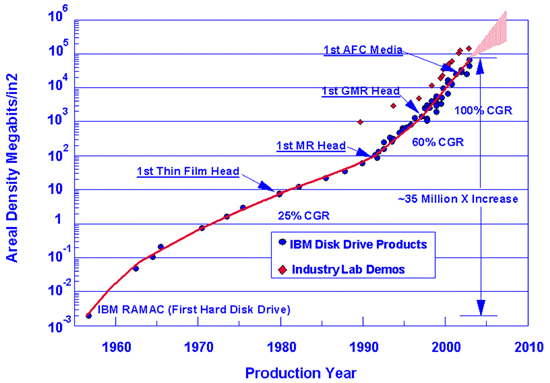
\includegraphics[width=75mm]{storage-density.png}

    \footnotesize DOI: 10.1081/E-ENN-120006100
\end{frame}

% TODO frame with Datta-Das transistor
\begin{frame}{Motivation - Perspectives of Spintronics}
    \begin{center}
    \textbf{Datta-Das Transistor}

    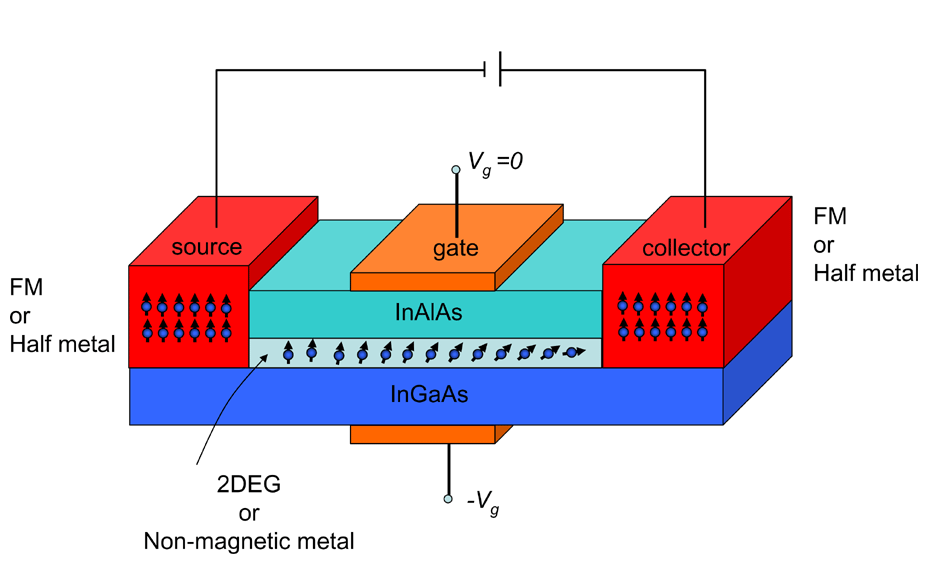
\includegraphics[width=8cm]{SpinFET.png}

    \vfill
    \footnotesize http://www.nims.go.jp/apfim/SpinFET.html
    \end{center}

\end{frame}

\begin{frame}{Disadvantages of Ferromagnetic Materials}

	\begin{itemize}
		\item Technologically hard to handle
        \item Limits in scaling down
        \item Static effects only
		\item Ferromagnetic materials are metals
            $\Rightarrow$ Schottky junctions when mixing with semiconductors
	\end{itemize}
\end{frame}

\subsection{Non-magnetic semiconductors}
\begin{frame}{Motivation - Alternatives}
    \textbf{Spin manipulation in non-magnetic semiconductors}

	\begin{itemize}
		\item Well-known techniques applicable
        \item Asymmetry tunable by electric fields
        \item Analogy to optics
	\end{itemize}
\end{frame}

\section{Theory}
\subsection{Relativistic quantum theory}
\begin{frame}{Theory: Pauli Equation}
    Relativistic QM in vacuum

    \begin{align*}
        \left( \frac{\vec p^2}{2m}- \frac{e\hbar \ \vec\sigma \cdot (\vec p \times \vec E)}
                        {2\Delta} +\ldots\right)\Psi = E \Psi
    \end{align*}

    \begin{align*}
        \Delta\qquad       & m_e c^2\\
        \vec \sigma \qquad & \textnormal{Pauli matrices}\\
        \vec p      \qquad & \textnormal{momentum}\\
        \vec E      \qquad & \textnormal{electric field}\\
    \end{align*}

\end{frame}

\subsection{Rasbha spin-orbit coupling}

\begin{frame}{Theory:  Bychkov-Rashba term}
    In Solids

    \begin{align*}
        H = \frac{\vec p^2}{2 m^*} + \alpha (\vec I \times \vec \sigma) \cdot
        \vec p
    \end{align*}

    \begin{align*}
        \alpha  \qquad & \textnormal{SO-coupling strength}\\
        \vec I  \qquad & \textnormal{Unit vector of asymmetry}
    \end{align*}

\end{frame}

\begin{frame}{Theory: Dispersion relation and Rashba}

    \begin{multicols}{2}
        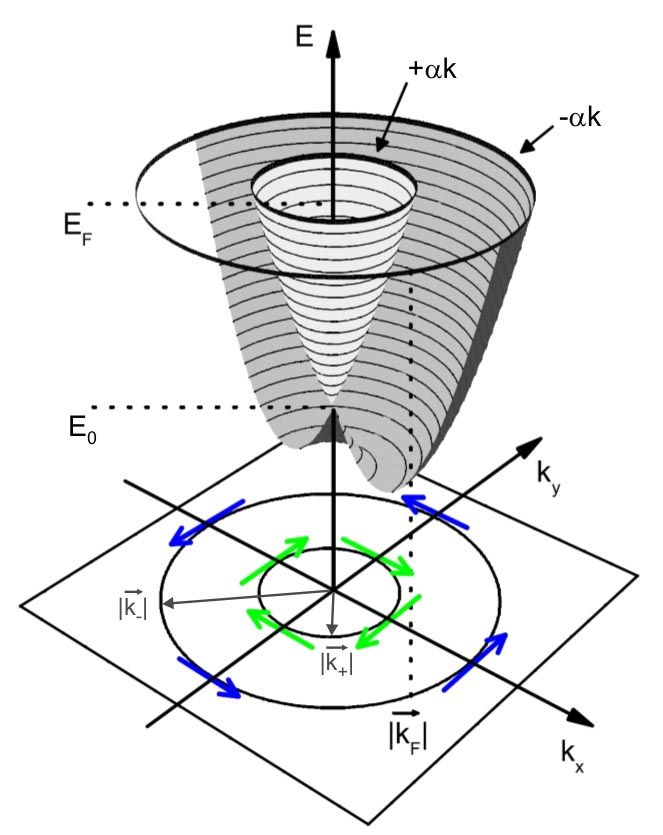
\includegraphics[height=6cm]{rashba-dispersion.jpg}

        \begin{align*}
            E(k) = \frac{\hbar^2}{2 m^*} k^2 \pm \alpha k
        \end{align*}

        Energy depends on spin and momentum $\Rightarrow$ manipulable\\[1em]

        $\alpha$ tunable through external electric field.
\end{multicols}
\end{frame}

\subsection{Landauer Formula}

\begin{frame}{Theory: Landauer Formula}
    \begin{multicols}{2}
        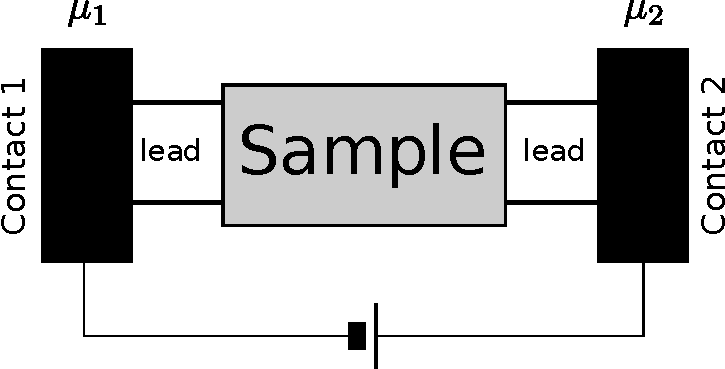
\includegraphics[width=6cm]{sample-leads}

        \begin{align*}
            G = \frac{2 e^2}{h} MT
        \end{align*}

        \begin{align*}
            G \qquad& \textnormal{conductance}\\
            M \qquad& \textnormal{number of modes}\\
            T \qquad& \textnormal{transmission propability}
        \end{align*}
    \end{multicols}
\end{frame}

%\begin{frame}{Theory: Green's Function formalism}
%    \begin{multicols}{2}
%        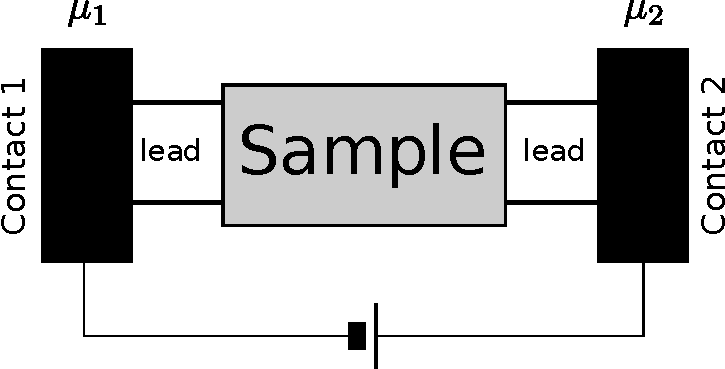
\includegraphics[width=6cm]{sample-leads}
%
%        \begin{align*}
%            G = \frac{2 e^2}{h} MT
%        \end{align*}
%
%        \begin{align*}
%            G \qquad& \textnormal{conductance}\\
%            M \qquad& \textnormal{number of modes}\\
%            T \qquad& \textnormal{transmission propability}
%        \end{align*}
%    \end{multicols}
%\end{frame}

\begin{frame}{Theory: Green's Functions}
    \begin{center}
        Inhomogeneous Schrödinger equation
        \begin{align*}
            (E-H) \Psi &= \delta(x-x_0)\\
            \Psi       &= \underbrace{(E-H)^{-1}}_{G} \delta(x-x_0)
        \end{align*}
        \pause
        \begin{align*}
            G^R = ((E + i \eta) -H)^{-1}\quad & \textnormal{Retarded Green's
            function}\\
            \qquad & \textnormal{wave moving away from exitation}\\
            G^A = ((E - i \eta) -H)^{-1}\quad & \textnormal{Adveanced Green's
            function}\\
            \qquad & \textnormal{wave moving towards exitation}
        \end{align*}

        \begin{align*}
        \end{align*}
   \end{center}
\end{frame}

\begin{frame}{Theory: Discretization}
    Problem: $(E\pm i\eta-H)$ is an operator, and not easily invertible\\[1em]

    \pause
    Solution: discretize derivatives into finite differences\\[1em]

    \pause
    Leads: Analytical Green's functions known\\[1em]

    \pause
    Describe coupling between leads and sample by matrices $\Sigma_p$
\end{frame}

\begin{frame}{Theory: Fisher-Lee Relation}
    {
        \huge
        \begin{align*}
            T_{pq} = \textnormal{Trace}( \Sigma_p G^R \Sigma_q G^A )
        \end{align*}
    }
    \begin{align*}
        \Sigma_p\qquad &\textnormal{Self-Energy matrix for lead $p$}\\
        G^R     \qquad &\textnormal{Retarded Green's function}\\ 
        G^A     \qquad &\textnormal{Advanced Green's function}\\ 
    \end{align*}
\end{frame}

\section{Work done}
\begin{frame}{Model}
    \begin{itemize}
        \item 2D electron gas in quantum well
        \item 2 bands considered
        \item $T = 0K$
        \item size: about 200nm
        \item ballistic transport
        \item coherent transport
        \item Interface between "normal" (N) and Spin-orbit  coupling (SO) regimes
    \end{itemize}
\end{frame}

\subsection{Analytical calculations}

\begin{frame}{Analytical calculations}
    \begin{multicols}{2}
        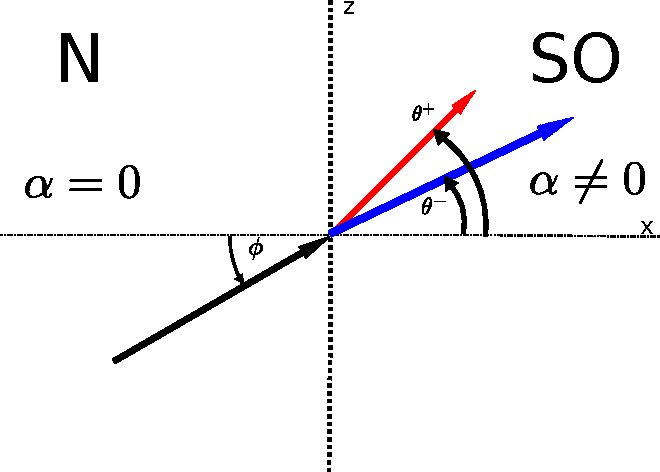
\includegraphics[width=55mm]{setup-simple}

        \begin{minipage}{0.5\textwidth}
            \textbf{N}: Normal regime, $\alpha = 0$\\
            \textbf{SO}: Spin-orbit coupling regime, $\alpha \not= 0$
        \end{minipage}

    \begin{align*}
        H_r &= \frac{p^2}{2m} + (-\vec y \times \vec \sigma) \cdot
                \alpha(x) \vec p\\ 
        E_{\pm} &= \frac{p^2}{2m} \pm \alpha \\
        v_{\pm} &= \frac{\partial E_{\pm}}{\partial p} = \frac{p}{m} \pm \alpha
    \end{align*}

    $\vec \sigma$ is the vector of Pauli matrices and describes the Spin

    \end{multicols}
\end{frame}


\begin{frame}{Analytical calculations - Eigenstates}
    \begin{align*}
    \chi_{SO}^{\pm} &= \frac{1}{n^{\pm}} 
                        \vect{-p_{x}^{\pm} \pm p^\pm}{p_z} \\
        n_{SO}^{\pm}   &= \sqrt{|-p_{x}^{\pm} \pm p^\pm|^2 + p_z^2}
    \end{align*}
\end{frame}
\begin{frame}{Analytical calculations - Wave Function}
    \begin{align*}
        \Psi^+ = e^{i p_z z} * \left\{
            \begin{array}{ll}
                e^{i p_x x} \chi_N^+ + e^{- i p_x x} (\chi_N^+ r_{++} +
                        \chi_N^- r_{-+})    & x < 0\\
                e^{i p_x^+ x} \chi_{SO}^+ t_{++} + e^{i p_x^- x}
                \chi_{SO}^- t_{-+}          & x > 0
            \end{array} \right.
    \end{align*}

    \begin{align*}
        r_{\pm+} \qquad & \textnormal{Reflection coefficients}\\
        t_{\pm+} \qquad & \textnormal{Transmission coefficients}
    \end{align*}

\end{frame}

\begin{frame}{Transmission coefficients}
    \begin{center}
        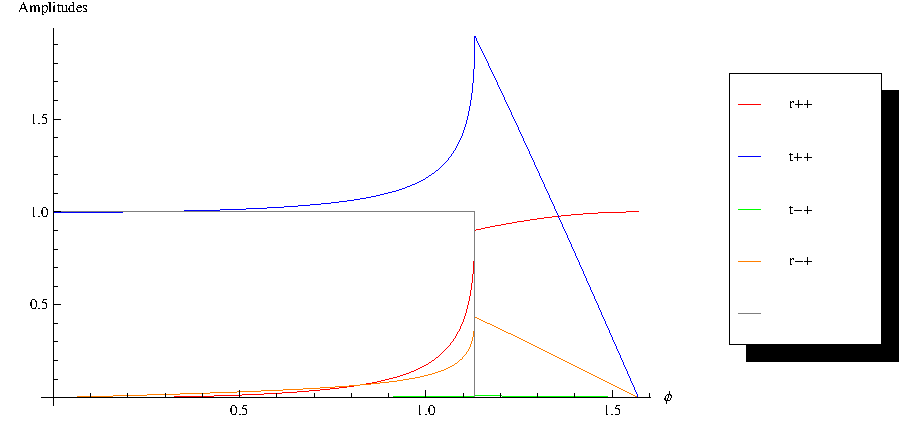
\includegraphics[width=10.0cm]{zero-plus.pdf}

        For $\phi > \phi_C$ the $e^{i p_{x,SO}^+ x }$ part vanishes
    \end{center}
\end{frame}

\begin{frame}{Critical angle for $+$ wave}
    \begin{center}
        \begin{align*}
            \phi_c          &= -\sin ^{-1}\left(\ta-\sqrt{\ta^2+1}\right)
        \end{align*}

        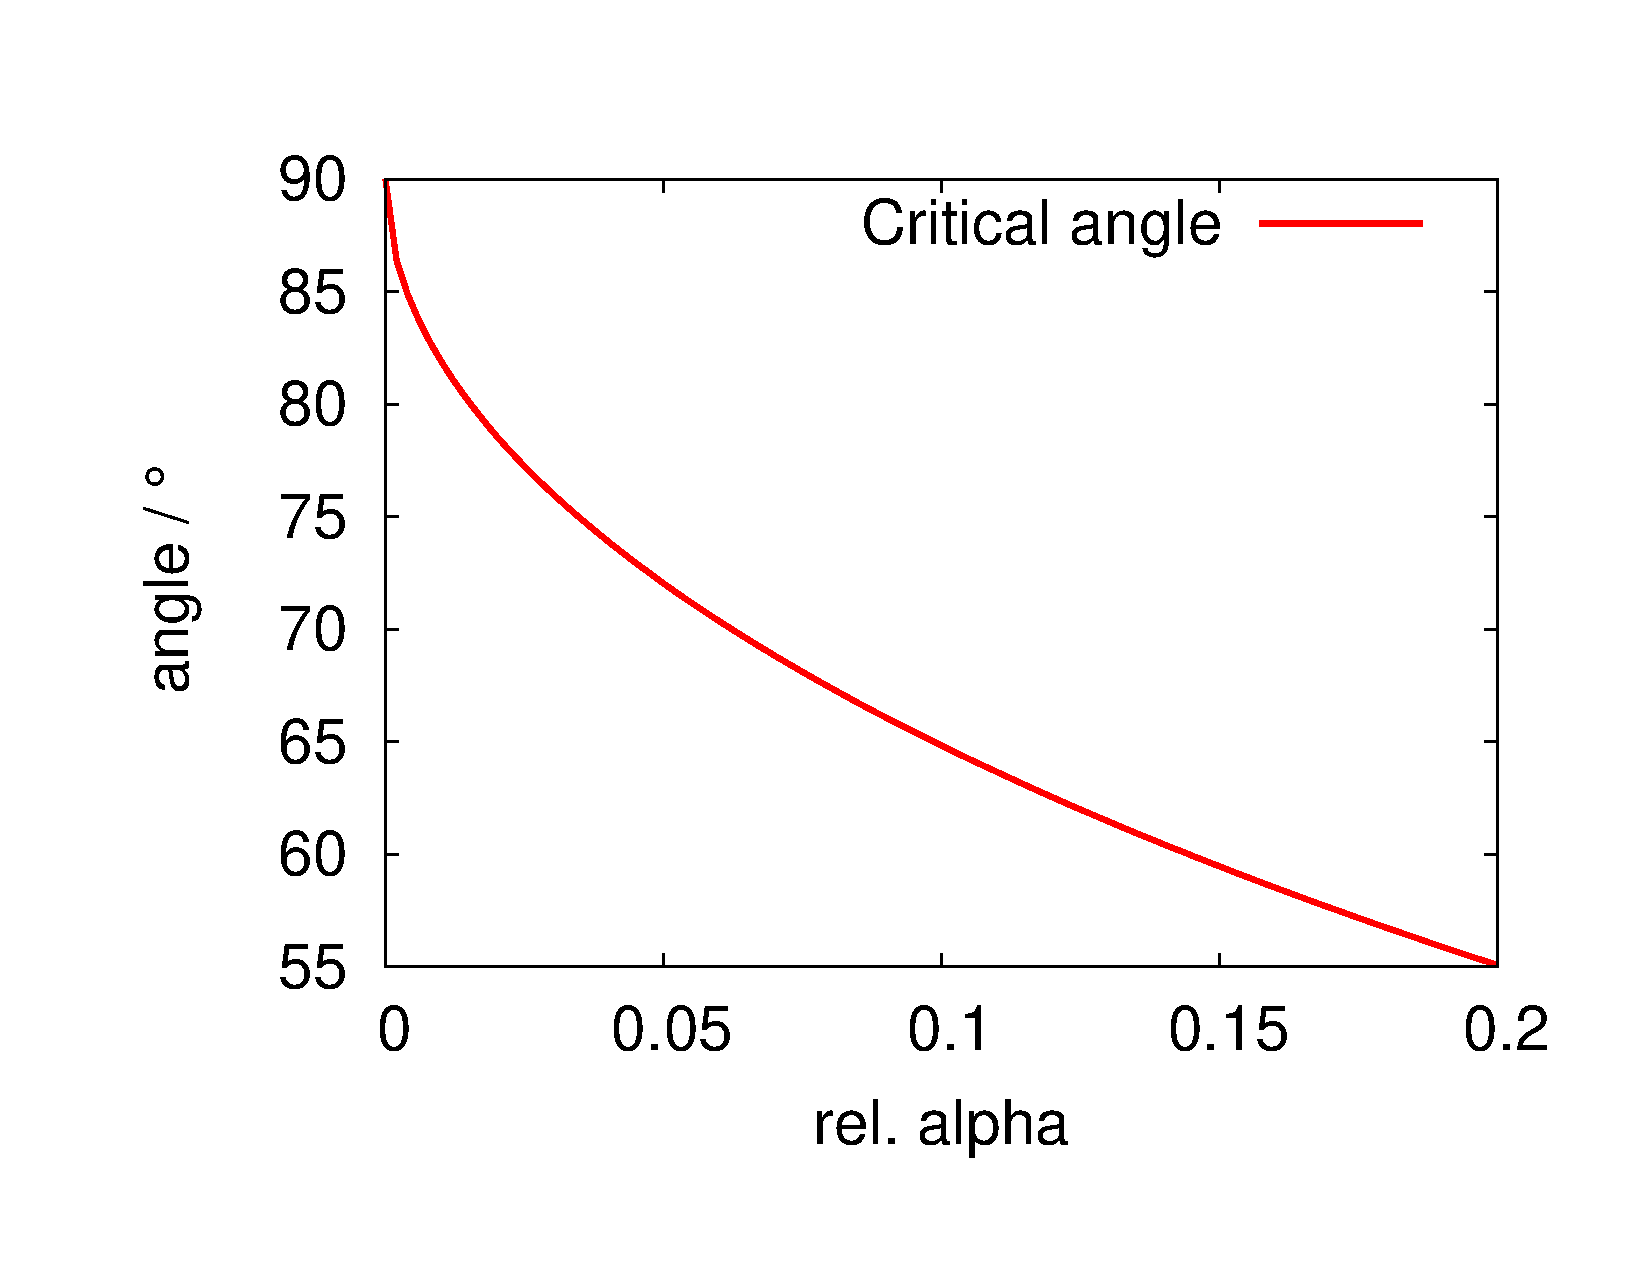
\includegraphics[width=0.7\textwidth]{critical-angle.pdf}
    \end{center}
\end{frame}

\begin{frame}{Figure of merit: Spin polarization}
    Each lead is assumed to consist of a spin-up ($\uparrow$) and a
    spin-down ($\downarrow$) sub-lead\\[2em]

    {
        \huge
        \begin{align*}
            T_S = T_{2\uparrow, 1\uparrow} + T_{2\uparrow, 1\downarrow}
            - T_{2\downarrow, 1\uparrow} - T_{2\downarrow, 1\downarrow}\\
        \end{align*}
    }

    $T_S$: Spin polarization perpendicular to the plane of 2-dimensional
    electron gas

\end{frame}

\begin{frame}{Adapting to $\uparrow, \downarrow$ bases}
    \begin{center}
        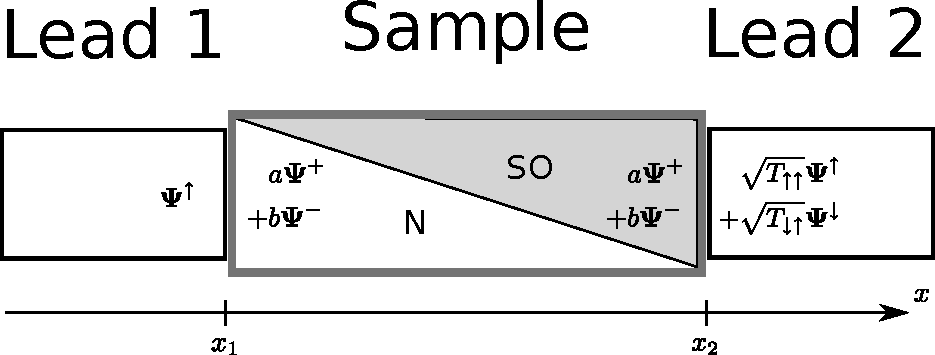
\includegraphics[width=\textwidth]{adapting-pic.pdf}
        \begin{align*}
            T_{2\uparrow,1\uparrow} = \left| \left( 
                a \mathbf{\Psi^+}(x=x_2) + b  \mathbf{\Psi^-}(x=x_2)
            \right)^\dagger \cdot \mathbf{\Psi}^\uparrow(x=x_2) \right|^2\nonumber\\
            T_{2\downarrow,1\uparrow} = \left| \left( 
                a \mathbf{\Psi^+}(x=x_2) + b  \mathbf{\Psi^-}(x=x_2)
            \right)^\dagger \cdot \mathbf{\Psi}^\downarrow(x=x_2) \right|^2\nonumber
        \end{align*}
    \end{center}

\end{frame}

\begin{frame}{What survives...}
    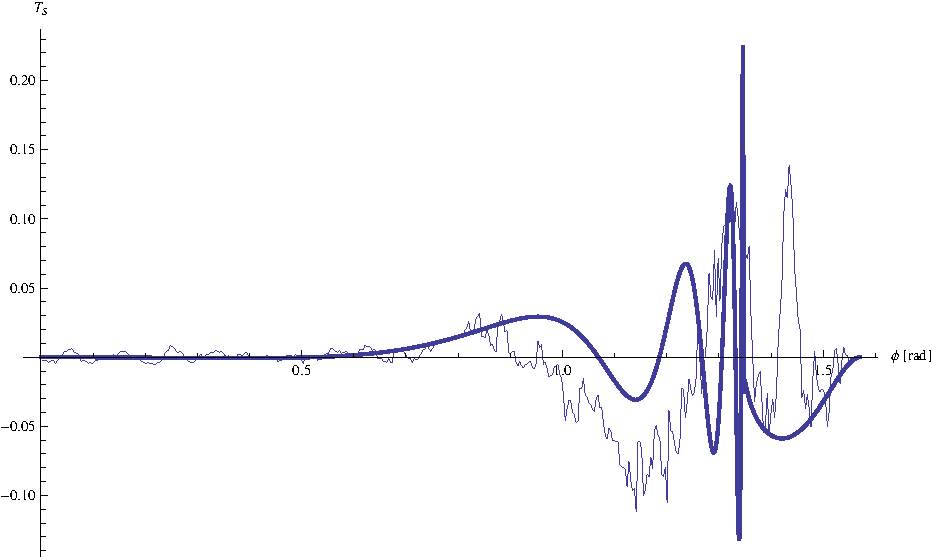
\includegraphics[width=\textwidth]{comparison-over-phi.pdf}
\end{frame}

\begin{frame}{Limits of analytical calculations}

    \begin{center}
    \begin{itemize}
        \item Limited to a single mode (typically 8 to 12 in experiment)
        \item Limited to simple geometry
        \item Hard to incorporate scattering centers, boundary conditions,
            finite size effects
    \end{itemize}
    \end{center}

\end{frame}

\subsection{Numerical calculations}
\begin{frame}{Numerical Calculations - The Plan}
    \begin{center}
    \begin{itemize}
        \item set up the Hamiltonian $H$
        \item calculate the self-energy matrices $\Sigma_p$
        \item calculate the Green's functions $G^A$ and $G^R$ by inverting
            $H + \sum_p \Sigma_p$
        \item use the Fisher-Lee relation to calculate the transmission matrix $T$
                from $G^R$, $G^A$ and $\Sigma_p$
    \end{itemize}
    \end{center}
\end{frame}

\begin{frame}{Enumerating sites}
    \begin{multicols}{2}
        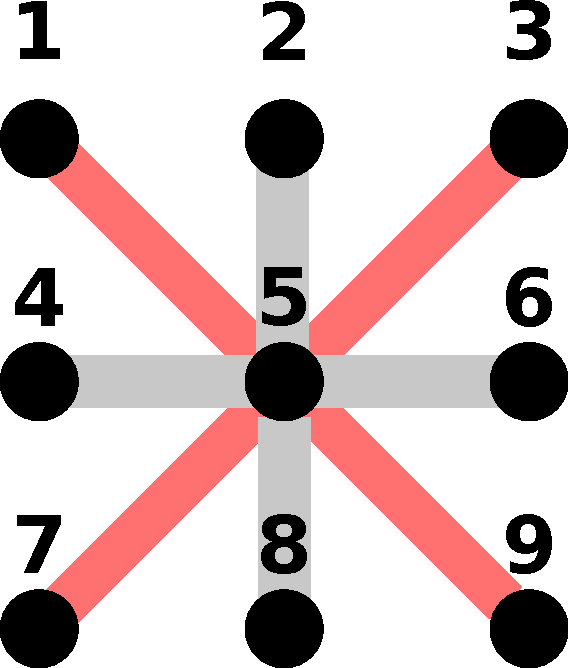
\includegraphics[width=0.4\textwidth]{hopping.pdf}
        \bf

        Gray: nearest neighbor hopping\\[1.5em]

        Red: next-nearest neighbor hopping (Rashba)\\[1.5em]

        Discretization lattice is \emph{not} the crystal lattice
    \end{multicols}
\end{frame}

\begin{frame}{Hamiltonian (1/3)}
    \small
    \begin{align*}
        H_{kin} &= \inp{
            \begin{array}{ccccccccc}
                -4t & t &  & t\\
                t & -4t & t &  & t &  &  & 0\\
                & t & -4t & 0 &  & t\\
                t &  & 0 & -4t & t &  & t\\
                & t &  & t & -4t & t &  & t\\
                &  & t &  & t & -4t & 0 &  & t\\
                &  &  & t &  & 0 & -4t & t\\
                & 0 &  &  & t &  & t & -4t & t\\
                &  &  &  &  & t &  & t & -4t\end{array}
        } \\
    \end{align*}
\end{frame}
\begin{frame}{Hamiltonian (2/3)}
    \footnotesize
    \begin{align*}
        H_{spin} &= \inp{
            \begin{array}{ccccccccc}
                0 & -\tso &  & i\tso\\
                \tso & 0 & -\tso &  & i\tso &  &  & 0\\
                & \tso & 0 & 0 &  & i\tso\\
                -i\tso &  & 0 & 0 & -\tso &  & i\tso\\
                & -i\tso &  & \tso & 0 & -\tso &  & i\tso\\
                &  & -i\tso &  & \tso & 0 & 0 &  & i\tso\\
                &  &  & -i\tso &  & 0 & 0 & -\tso\\
                & 0 &  &  & -i\tso &  & \tso & 0 & -\tso\\
                &  &  &  &  & -i\tso &  & \tso & 0
            \end{array}
        }
    \end{align*}
\end{frame}

\begin{frame}{Hamiltonian (3/3)}
    \begin{center}
        \begin{align*}
            H &= \inp{
            \begin{array}{cc}
                    H_{kin}  & H_{spin} \\
                    H_{spin}^\dagger & H_{kin} \\
            \end{array}}
        \end{align*}
    \end{center}

    System size: $n \times n$

    Matrix size: $2n^2 \times 2n^2$

    System: $150 \times 150 \Rightarrow 2.025 \cdot 10^9$ matrix entries.

    Double precision floating point number: 64 bit = 8 byte

    $\Rightarrow \approx 16$GB memory per matrix

\end{frame}

\begin{frame}{Interface}
    \begin{center}
        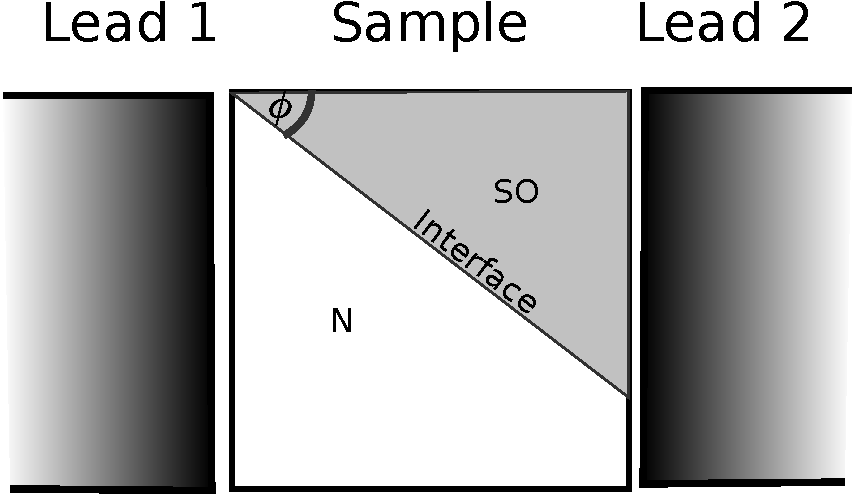
\includegraphics[width=0.5\textwidth]{sample-lead-interface.pdf}%
        \hspace{0.1\textwidth}%
        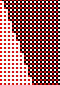
\includegraphics[width=0.2\textwidth]{hopping.png}
    \end{center}
\end{frame}

\begin{frame}{Results - Rashba Precession}
    \begin{center}
        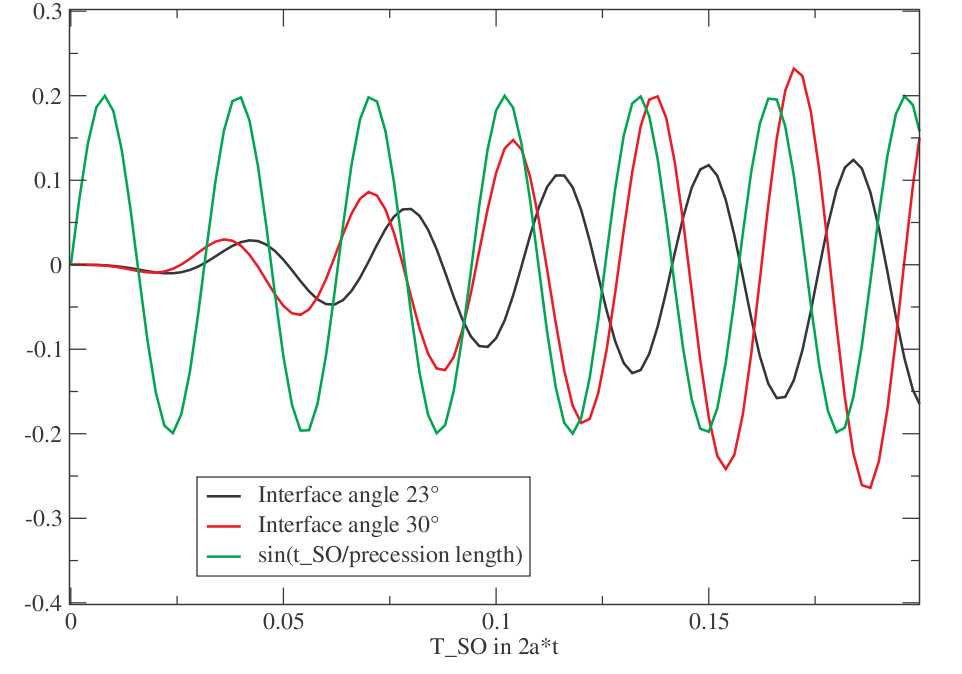
\includegraphics[width=0.8\textwidth]{interface-precession.png}
    \end{center}
\end{frame}

\begin{frame}{Results - Spin Polarization}
    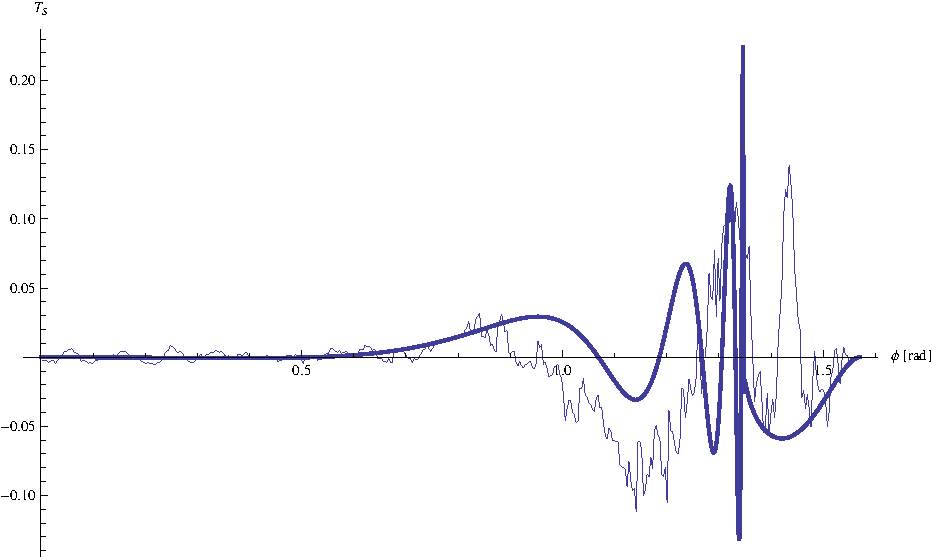
\includegraphics[width=0.8\textwidth]{comparison-over-phi.pdf}
\end{frame}

\begin{frame}{Results - Comparison}
    \begin{multicols}{2}
    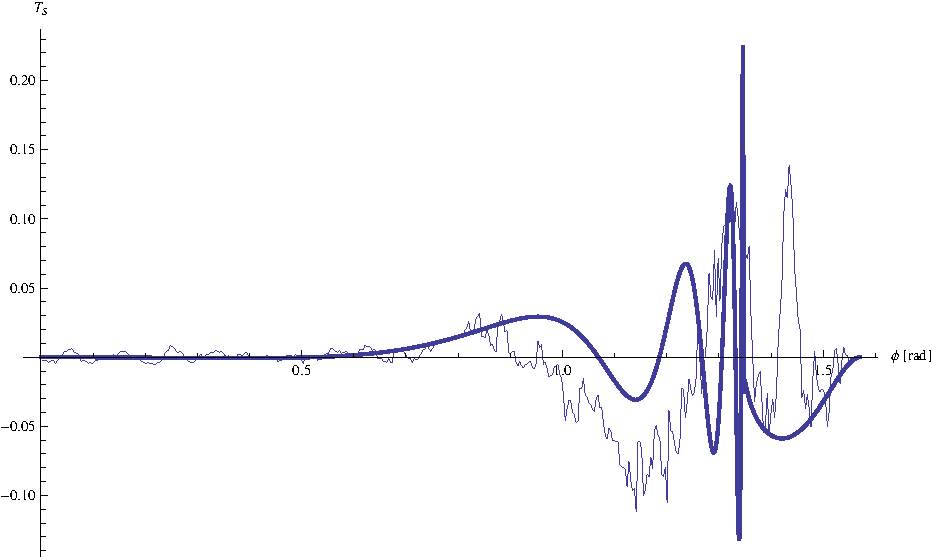
\includegraphics[width=0.5\textwidth]{comparison-over-phi.pdf}

    Rough interface leads to noise\\[1em]

    Number of modes varies in simulation\\[1em]

    Angle between beams and leads leads to reflection

    \end{multicols}
\end{frame}

\begin{frame}{Results - Two non-zero SO Strengths}
    \begin{center}
        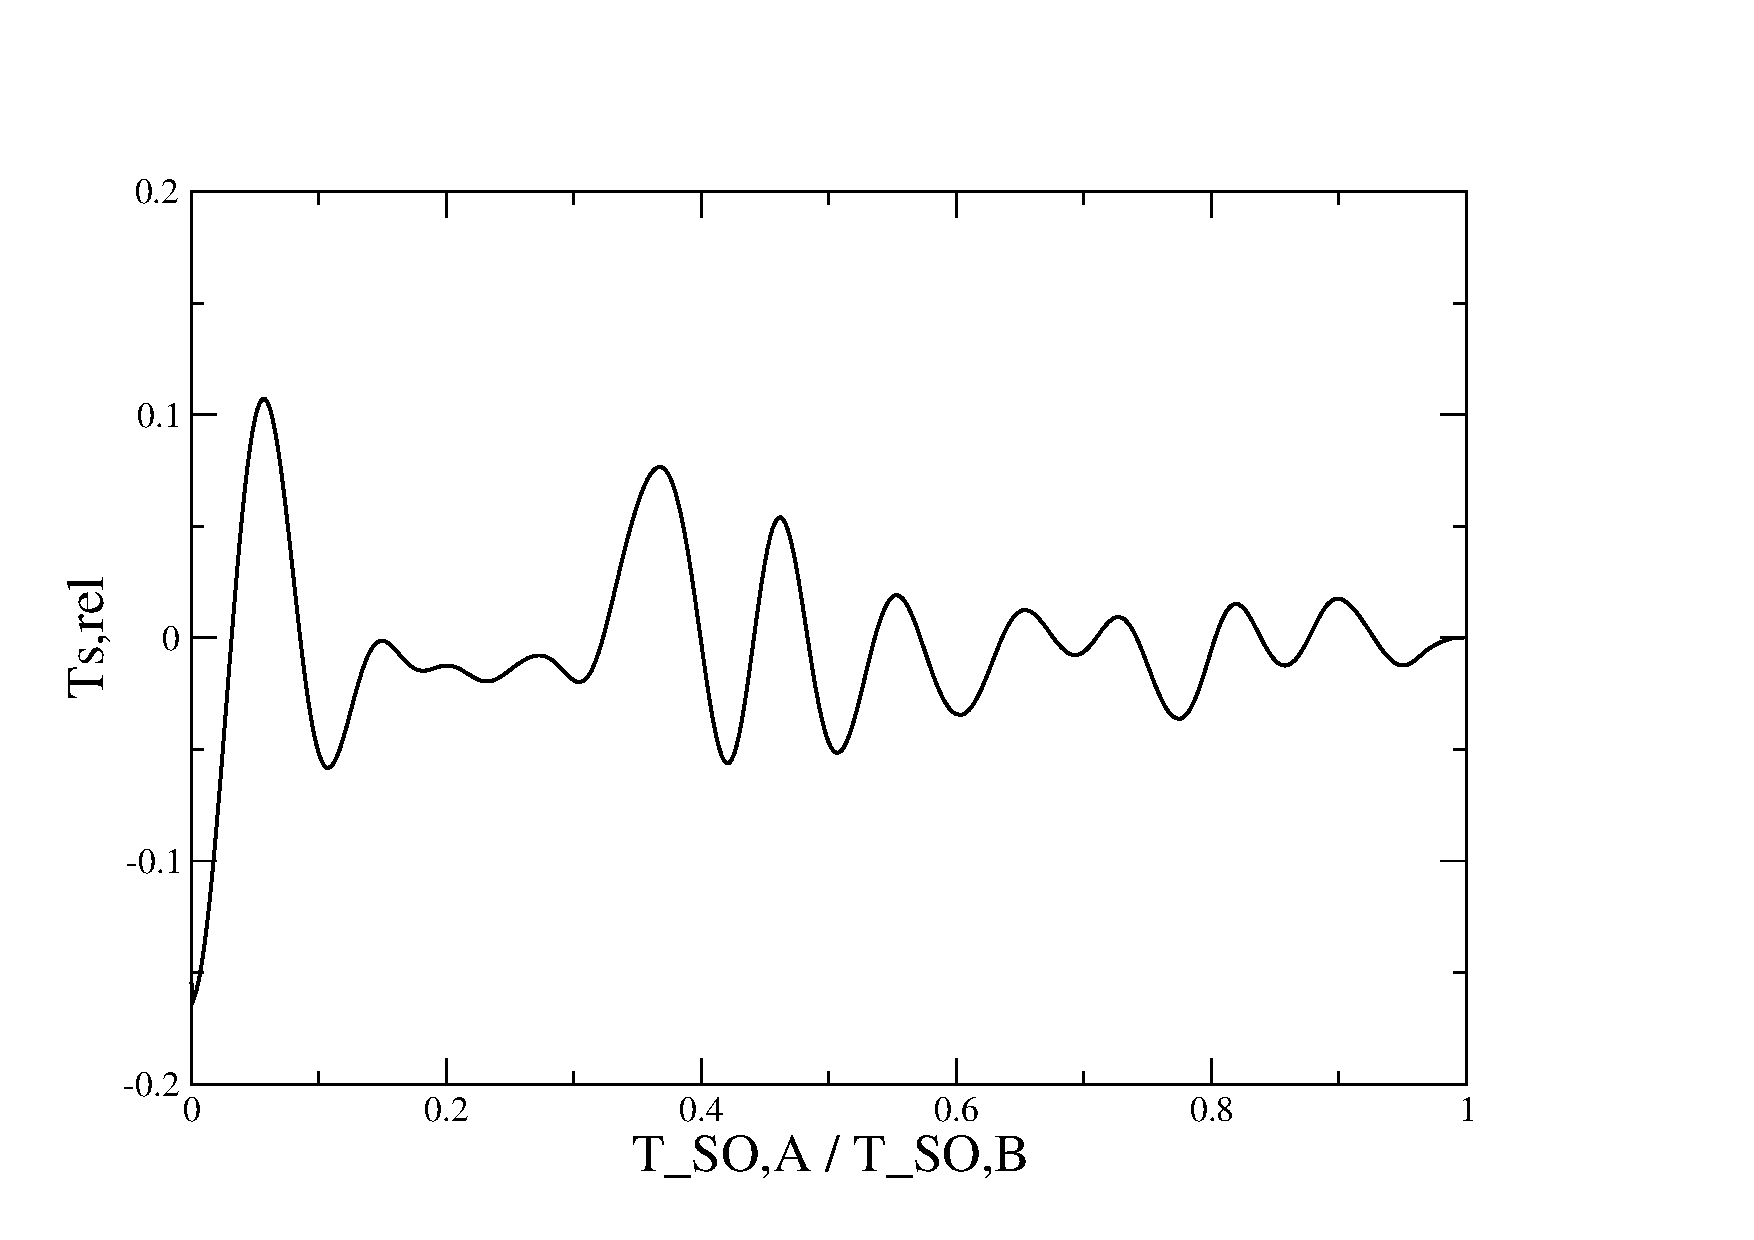
\includegraphics[width=0.7\textwidth]{polarization-so-so-rel.pdf}

   Relative spin polarization $T_s^{rel}$ as function of
        $ \frac{\tso{}_A}{\tso{}_B} =\frac{\ta_A}{\ta_B}$

        For a fixed $\phi=80^\circ$ and $\tso{}_B = 0.1$.

    \end{center}
\end{frame}

\begin{frame}{Experimental Realisation}
    \begin{center}
        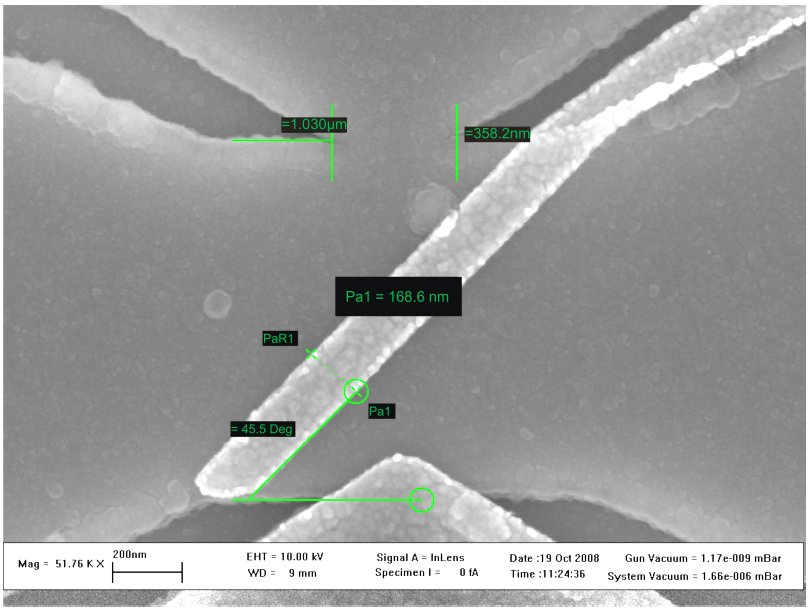
\includegraphics[width=0.7\textwidth]{beamsplitter2.jpg}

        M. Mühlbauer, Institut für Experimentelle Physik, Würzburg
    \end{center}
\end{frame}

\section{Summary}

\begin{frame}{Summary}
    \begin{itemize}
        \item Spintronics is a successful and interesting field (GMR,
            Datta-Das transistor)
        \item Rashba SO-Coupling: spin filtering with critical phenomena
        \item Up to $20\%$ spin separation
        \item rough agreement between analytical and numeric calculations
        \item Generalization to two different SO regions
    \end{itemize}

\end{frame}

\end{document}
